\documentclass{article}
\usepackage[utf8]{inputenc}
\usepackage{amsmath}
\usepackage{amsfonts}
\usepackage{mathrsfs}
\usepackage{graphicx}
\usepackage{subcaption}
\usepackage[top=30truemm,bottom=30truemm,left=30truemm,right=30truemm]{geometry}


\title{Chaotic Dynamics: Homework 5}
\author{Kansuke Ikehara (Kansuke.Ikehara@colorado.edu)}

\begin{document}
\maketitle

\subsection*{Problem 2}
\subsubsection*{(a)}
Fig.\ref{q2a} depicts a chaotic attractor of the Lorenz system, which is calculated by the adaptive RK4 solver.
\begin{figure}[h]
  \centering
  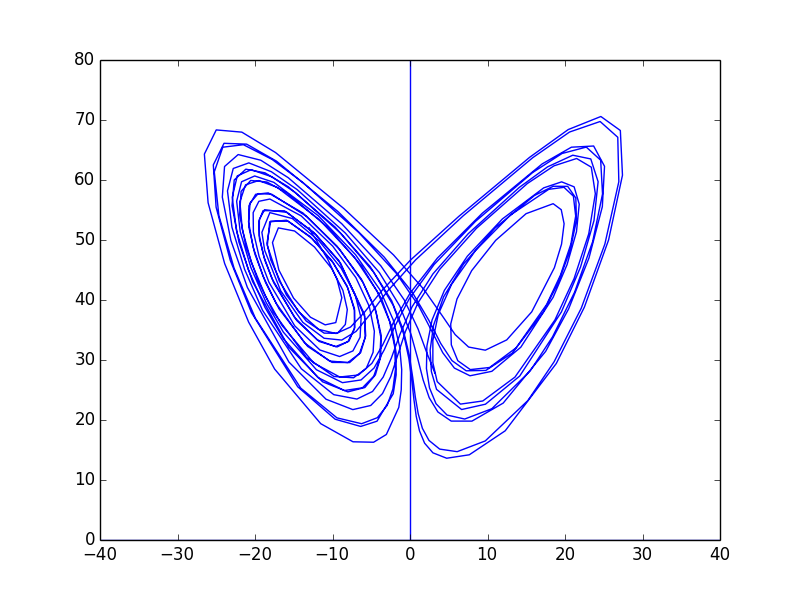
\includegraphics[height=2in]{figs/q2a/adaptive_1_n500.png}
  \caption{chaotic attractor of the Lorenz system}
  \label{q2a}
\end{figure}

\subsubsection*{(b)}
Fig.\ref{q2b} shows the partial plots of the attractor of Lorenz system calculated by adaptive and nonadaptive RK4 solvers, respectively. Blue dots are trajectories derived by adaptive RK4 solver and red dots are the ones from non-adaptive RK4 solver. Those two solutions generally agree with each other around the early stage, but gradually deviate a bit from one another as time goes as seen in the right half. Space between in points produced by adaptive RK4 solver is not even over the course of action, which can been seen especially in the right side of the plot.
\begin{figure}[h] 
  \centering
  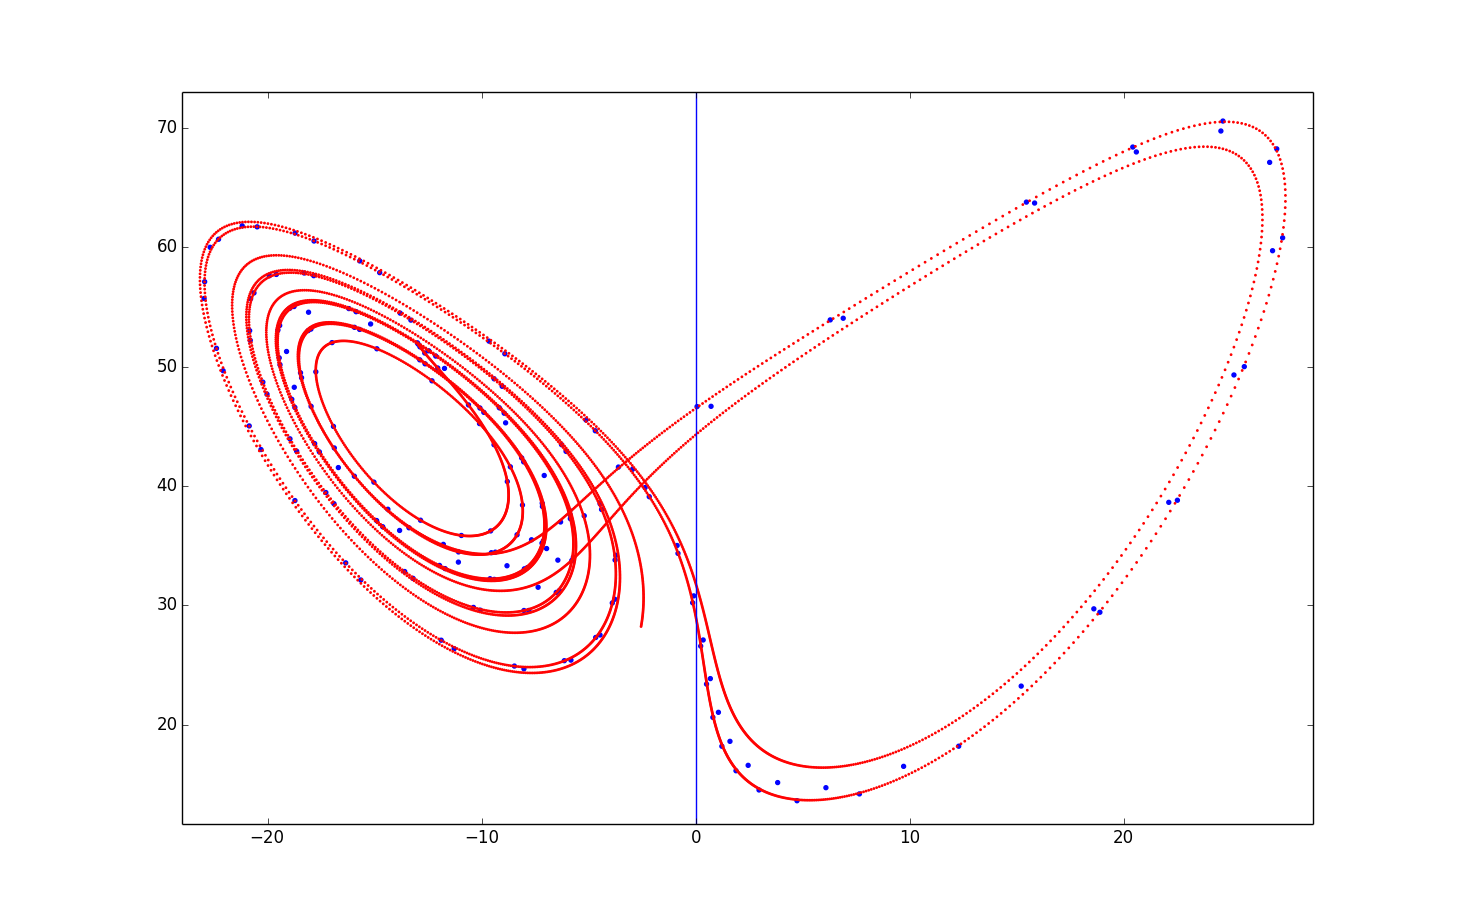
\includegraphics[height=2in]{figs/q2b/q2_b_comparison2.png}
  \caption{Overlaid trajectories}
  \label{q2b}
\end{figure}

\subsubsection*{(c)}
When $0 < r < 1$, the trajectory of the systems converges to zero regardless of the initial condition. This implies that the entire state space is the basin of an attractor, which is zero. When $13.5 < r < 14$, the trajectory interestingly behaves: depending on the initial condition, the trajectory converges to a fixed point spirally in either side of the x-axis. Since the Lorenz system is symmetric, those spirals are symmetric as well. When $23 < r < 29$, trajectory forms a spiral on a fixed point but the speed of convergence gets slower as $r$ increases. When $29 < r$, the trajectory looks quite a like chaotic orbit as we have seen in the questions above. 

\subsection*{Problem 3}
Fig.\ref{q3} shows the state-space trajectory of Rossler system in x-y projection. 
\begin{figure}[h] 
  \centering
  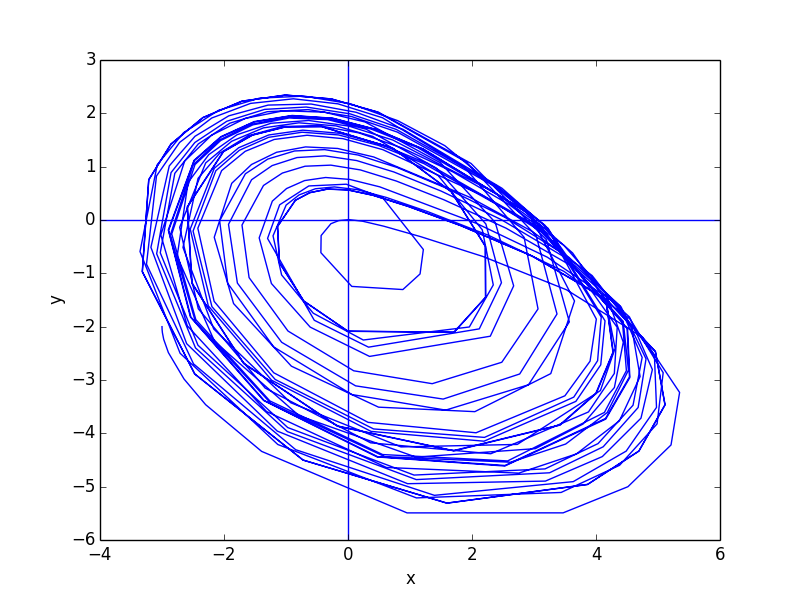
\includegraphics[height=2in]{figs/q3/fig.png}
  \caption{the trajectory of Rossler system}
  \label{q3}
\end{figure}

\subsection*{Problem 4}
Figs \ref{q4_1} and \ref{q4_2} show the state-space trajectories for error values 10 and 100, respectively. As allowed error value increases, the adaptive RK4 solver tends to increase the time step, resulting in overshoot and significant deviation from what it should follow. This is essentially the same effect as we saw in the previous problem set, where we have increased the time step $\Delta t$ for non-adaptive RK4 solver.
\begin{figure}
\centering
\begin{subfigure}{.5\textwidth}
  \centering
  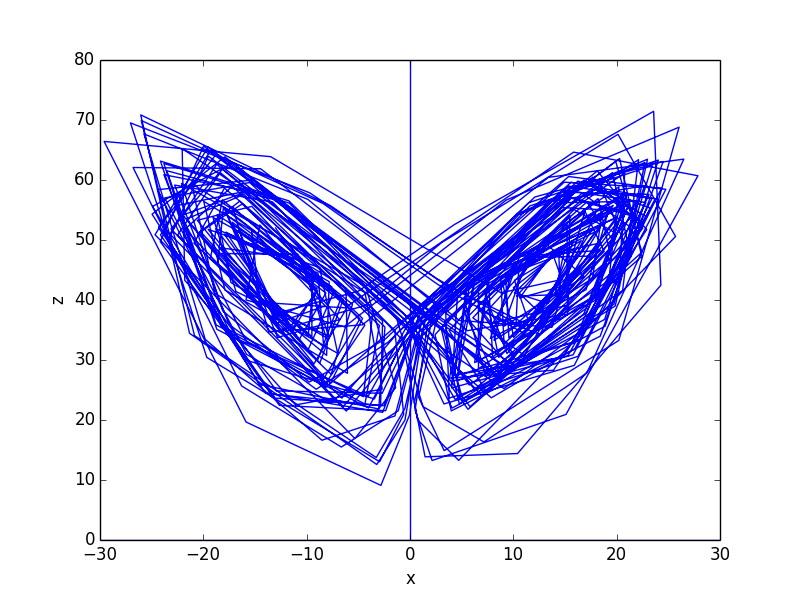
\includegraphics[height=2in]{figs/q4/err_10.png}
  \caption{error = 10}
  \label{q4_1}
\end{subfigure}%
\begin{subfigure}{.5\textwidth}
  \centering
  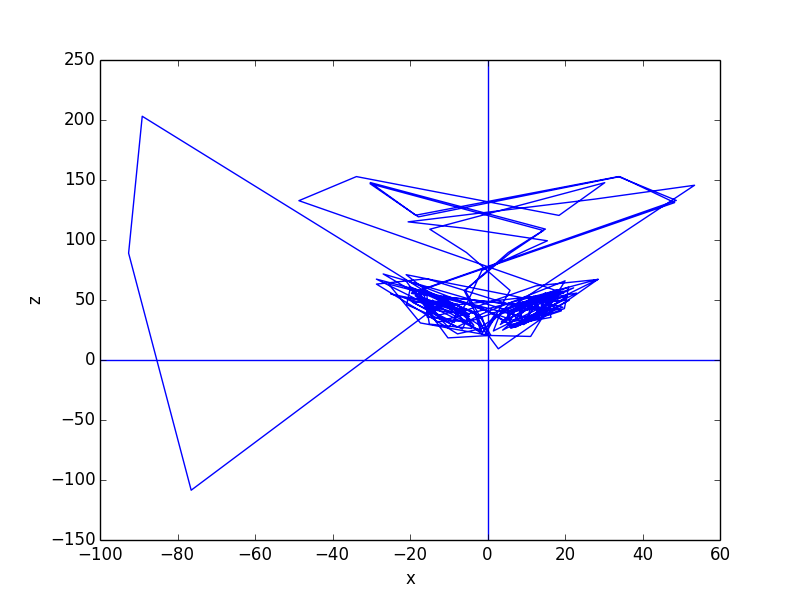
\includegraphics[height=2in]{figs/q4/err_100.png}
  \caption{error = 100}
  \label{q4_2}
\end{subfigure}
\caption{state-space trajectories for different error values.}
\label{q4}
\end{figure}

\end{document}












